\documentclass[10pt,twocolumn,letterpaper]{article}

\usepackage{cvpr}
\usepackage{times}
\usepackage{epsfig}
\usepackage{graphicx}
\usepackage{amsmath}
\usepackage{amssymb}
% \usepackage{natbib}
\usepackage{subcaption}

% Include other packages here, before hyperref.

% If you comment hyperref and then uncomment it, you should delete
% egpaper.aux before re-running latex.  (Or just hit 'q' on the first latex
% run, let it finish, and you should be clear).
\usepackage[pagebackref=true,breaklinks=true,letterpaper=true,colorlinks,bookmarks=false]{hyperref}
\newcommand{\matr}[1]{\mathbf{#1}} % undergraduate algebra version

\cvprfinalcopy % *** Uncomment this line for the final submission

\def\cvprPaperID{0001} % *** Enter the 3DV Paper ID here
\def\httilde{\mbox{\tt\raisebox{-.5ex}{\symbol{126}}}}

% Pages are numbered in submission mode, and unnumbered in camera-ready
%\ifcvprfinal\pagestyle{empty}\fi
%\setcounter{page}{4321}
\begin{document}

%%%%%%%%% TITLE
\title{Mapping Building Outlines to 3D Point Clouds}

\author{Anurag Sai Vempati\\
Autonomus Systems Lab\\ ETH Zurich\\
{\tt\small firstauthor@i1.org}
% For a paper whose authors are all at the same institution,
% omit the following lines up until the closing ``}''.
% Additional authors and addresses can be added with ``\and'',
% just like the second author.
% To save space, use either the email address or home page, not both
\and
Wolf Vollprecht\\
\\
\\
{\tt\small wolfv@student.ethz.ch}
}

\maketitle
%\thispagestyle{empty}

%%%%%%%%% ABSTRACT
\begin{abstract}
  While point clouds are easy to obtain through processes such as Structure-From-Motion they only exist in a space for themselves. GPS coordinates, recorded at capture time of the images, can give a sparse and noisy reference to the true position of the point cloud. In this paper we present a method to register a point cloud on reference map data.
\end{abstract}

%%%%%%%%% BODY TEXT
\section{Introduction}

With current state of  the art technology, obtaining point clouds through structure from motion has become an easy task. 
Several attempts deal with a similar problem, such as ... 

\section{Obtaining the ground truth}

\begin{figure}[h]
   \centering
   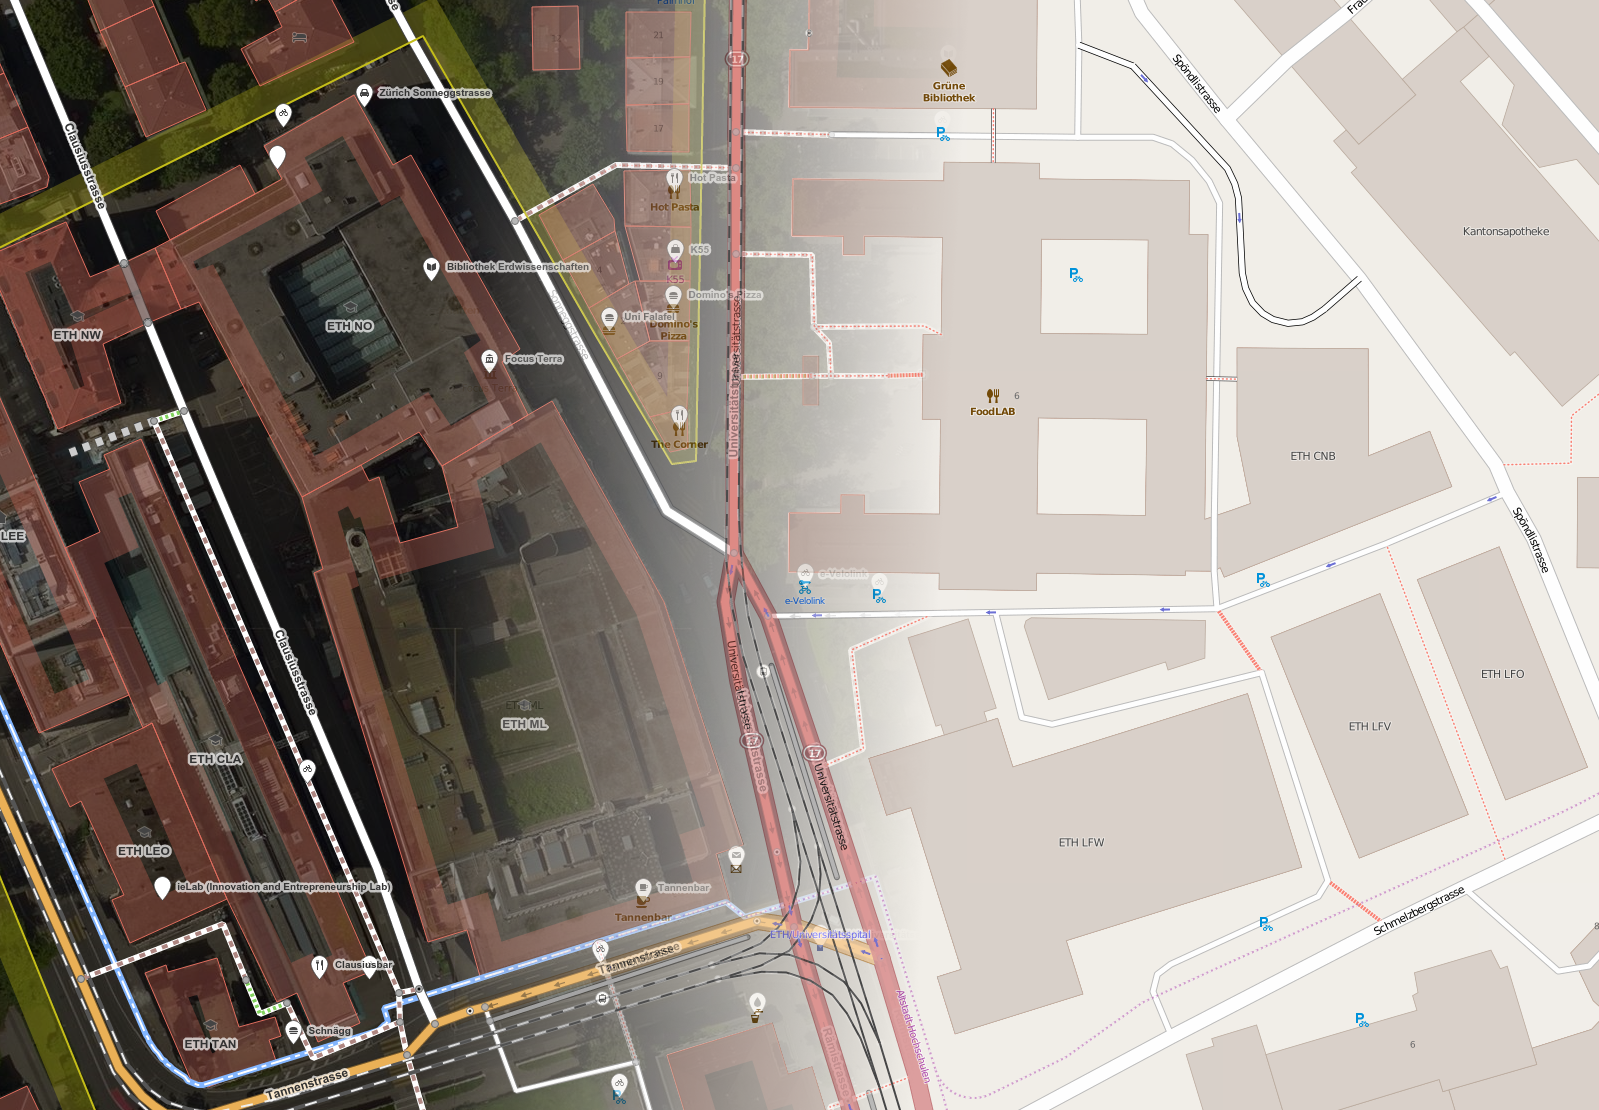
\includegraphics[width=\linewidth]{images/osm_map.png}
   \caption{OSM overlaid with editor interface}
   \label{fig:figure1}
\end{figure}


In order to obtain the ground truth building outlines, we used OpenStreetMaps\footnote{\url{http://www.openstreetmap.org/}}, a collaborative mapping effort that takes place globally. Volunteers are mapping their surroundings and upload it to a central database, where all changes to the map are stored. 
Of concern for us is only one mapped entity, the building. All points in OSM are stored as nodes. The entity consists of one or more node (in the case of a building it's multiple nodes). By parsing the XML response and mapping all node values to the corresponding building entity, we can obtain all corner points of the closed polygon that describes a building outline in the real world.

In order to adjust the point cloud to the obtained ground truth, we discretized the polygons to point clouds themselves by creating points along the polygon edges in a certain distance. During the Iterative Closest Point matching these points will be matched against the point cloud and provide an error distance.

The OSM data is in the standard latitude/longitude coordinate format. This representation maps coordinates to the globe, which has a spherical shape. However, we would like to work on a 2D surface. The size of the registration is reasonably small to obtain a 2D representation that falls into the boundaries of acceptable error.

There are a number of methods on how to convert coordinates to a 2D representation, which is a topic that has been explored for a long time since large-scale mapping has taken place globally. An exhaustive overview can be found in Snyder (1987)~\cite{Snyder1987}. The methods can be divided into two different categories:

\begin{itemize}
   \item \textbf{Conformal} This category of mappings preserves angles as observed in the real world (ie. the local angles are preserved). 
   \item \textbf{Equiareal} Retains equal area
   \item \textbf{Equidistant} Preserving distance
   \item \textbf{Azimuthal} Preserving Direction
   \item \textbf{Shortest Route} Shortest route is observable 
\end{itemize}

Since the sphere cannot be flattened out without distortion (ie. the sphere is a non-developable surface) not all of the above properties can hold for a projection at the same time.

For our application of registering a 2D point cloud on the map, we chose to use the Universal Transverse Mercator (UTM) projection, which preserves the angles and shapes, a property we deemed useful for our application.

Contrary to other map projections, UTM is not a single projection but rather divides the globe into 60 different zones.

\section{Registering the Point Cloud}

After obtaining the ground truth and the 2D projection of the 3D cloud we are now able to register the point cloud on the OSM reference.

Therefore we use ``Iterative Closest Point'' (ICP) matching algorithm. As the name suggest, ICP is an iterative algorithm to minimize the distance between two (or more) point cloud measurements. ICP is a widely used algorithm for example in robotics (Simultaneous Localization and Mapping [SLAM]). 

The input to the ICP algorithm in general is two pointclouds, one called the reference and the other source. The source should be aligned to the reference cloud. The output of the algorithm is a transformation matrix in 2 or 3 dimensions. Furthermore, the algorithm needs to be supplied with a stop condition, for example a maximum number of iterations or a minimal size of change between iterations, which indicates that the algorithm has converged to a minima.

Several important drawbacks of ICP are that it usually only provides rigid transformations (i.e. scale and shear factors are not affected). Allowing infinite scale the ICP solution would scale down to only one point with a distance of zero, as all points would be incident with that one. Another problem is that ICP, without good initialisation, tends to convertge to a local minima. Therefore it is paramount to have an initial rotation and translation that matches the reference somewhat. % We are currently able to do this based on the GPS positions in our source data which indicate a 

For our implementation, the existing \texttt{libpointmatcher}\cite{Pomerleau12comp} library was utilized to provide a framework for customizable ICP algorithms.

Both the map data as well as the point cloud is normalized and scaled to an arbitray scale, so that the leftmost point is coincident with the (0, 0) coordinate.

\subsection{ICP process}

As implemented, the ICP implementation uses a KD-Tree with a variable number of neighbors it considers as potential neighbors. The nearest neigbor is accepted as neighbor and a transformation is searched that decreases the distance (error) between all neighbors. 

Generally, there are two different popular ICP variants: Point-to-Point and Point-to-Plane, with the latter usually performing better. However, since we are operating in the 2D space, there are no planes except for the ground plane to be found. Thus we decided to use the more approachable point-to-point algorithm.

One ICP iteration consists of 4 steps:

\begin{itemize}
   \item We search a KD-Tree structure for the nearest neighbors and weight or reject them depending on the distance
   \item The error is calculated
   \item Using the error, the singular value decomposition (SVD) is calculated
   \item The rotation matrix is $\matr{R} =\matr{U} * \matr{V}^{\intercal}$
      \\ The translation vector is $\matr{T} = \matr{A} - \matr{R} * \matr{B}$
      \item Repeat process until either only a very small change between iterations is observed or the error is sufficiently small
\end{itemize}

\subsection{Filtering data}


\begin{figure}

\begin{subfigure}{.5\linewidth}
  \centering
  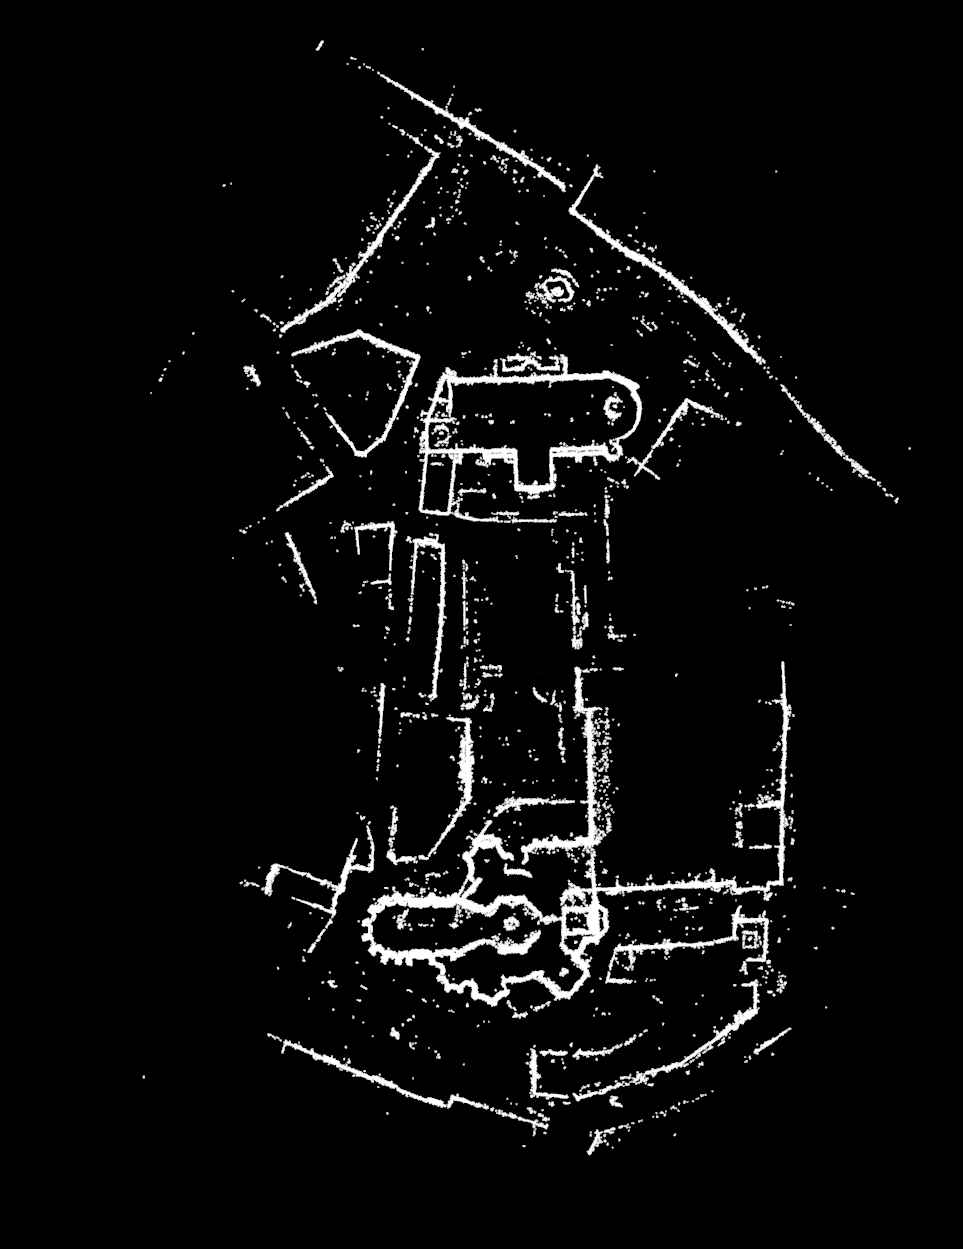
\includegraphics[width=.8\linewidth]{images/Selection_031.png}
  \caption{Original input}
  \label{fig:sfig1}
\end{subfigure}%
\begin{subfigure}{.5\linewidth}
  \centering
  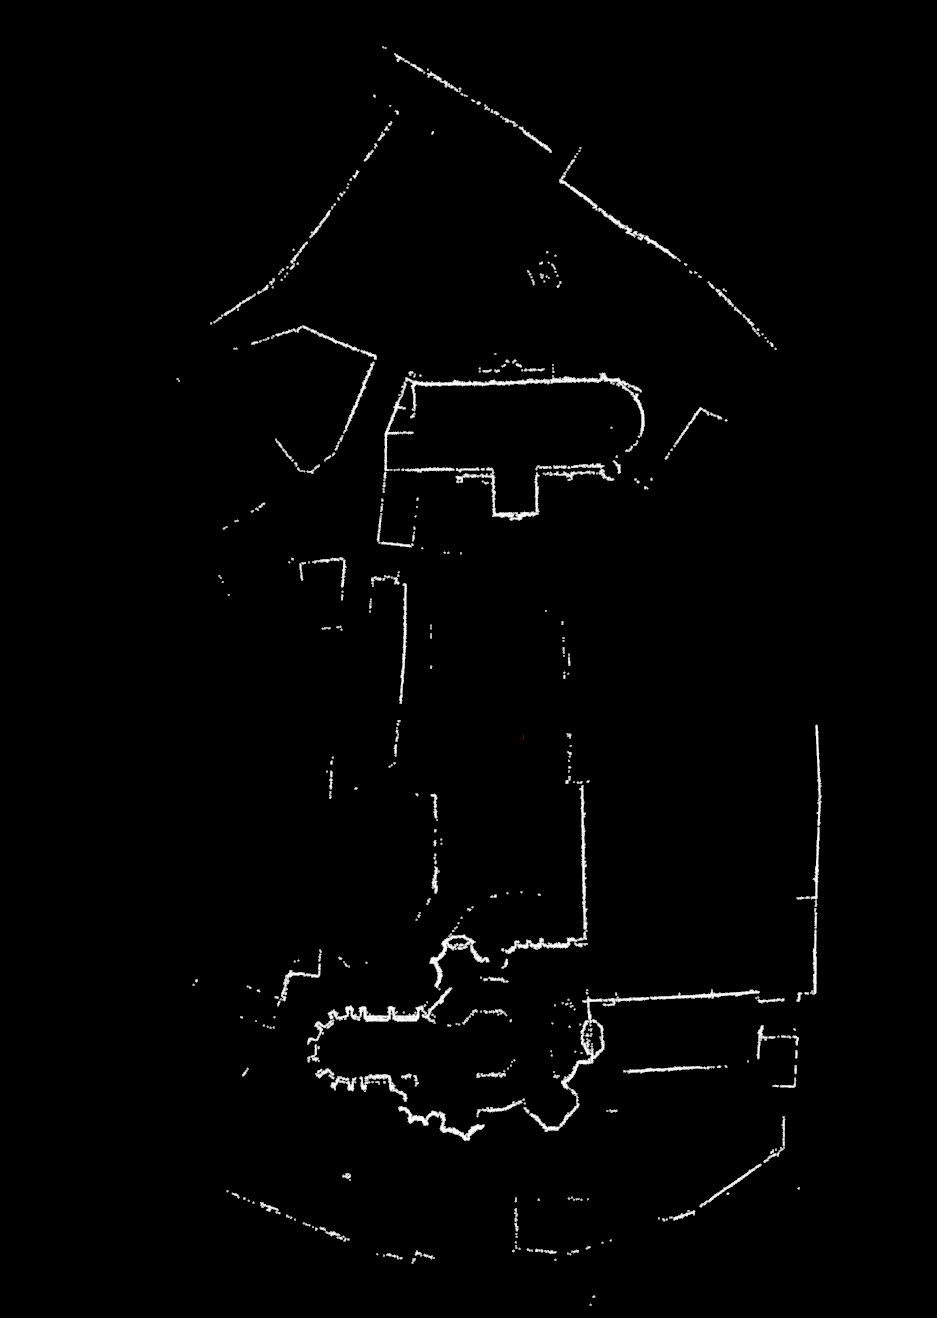
\includegraphics[width=.8\linewidth]{images/Selection_032.png}
  \caption{Output after filter}
  \label{fig:sfig2}
\end{subfigure}

\end{figure}


To further reduce the amount of noise, we implemented a filtering chain, consisting of 

\begin{itemize}
   \item Any given point needs at least 50 neighbors in a radius of 2 meters to be considered a valid measurement
   \item Statistical outliers are removed with a mean of 8 and a standard deviation of 1. This further removes outliers
   \item Only 1/8 of all remaining points are randomly chosen to reduce the computational load
\end{itemize}

\subsection{Initial alignment}

\begin{figure}
   \item 

\end{figure}

As stated before, the initial alignment of the two pointclouds is crucial for successful ICP matching. 
In order to find a good initial alignment, we try to find corner points in the measured data. 

There exist a number of corner detectors that are well researched. Some of the most notable ones, the Hough-transform~\cite{illingworth1988survey} and the Harris-detector~\cite{harris1988combined} were tried, but didn't deliver sufficient results. The properties of our data are also not extremely well suited for these algorithms which were primarily developed for images. 

We developed an approach based on the Random Sample Consensus algorithm (RANSAC)~\cite{fischler1981random}. RANSAC is able to detect lines in a robust way. Our process looks like this:

\begin{itemize}
    \item Choose random point from point cloud
    \item Select nearest 100 neighbors from kd-tree and insert into sub point cloud
    \item Find best line with RANSAC
    \item Remove all inliers from sub point cloud
    \item If more than threshold points remaining, find second best line by running RANSAC again
    \item Check angle between both lines (if angle to small or wide, reject)\footnote{Rejecting intersection points based on angle is possible for us since we are primarily interested in corners that meet at about 90 degree. This is due to the fact that we are working with city scapes.}
    \item If line is found, calculate intersection point
    \item Reject if intersection point is not close to points in sub point cloud
\end{itemize} 

After a certain, arbitray numbers of corners is found, we use the map of corners to match the OpenStreetMap data. Therefore we randomly select 3 points from the corner map, and calculate a corresponding transformation to three points on the OSM data. This makes it possible to calculate an error and improve or reject several initial transformations.

We then choose the best transformation and use it as intial transformation for the ICP.

{\small
\bibliographystyle{ieee}
\bibliography{egbib}
}


\end{document}
